%\section{Cálculo de magnitudes en equilibrio: Presión y temperatura}

% %\section{Cálculo de magnitudes en equilibrio: Presión y temperatura}

% %\section{Cálculo de magnitudes en equilibrio: Presión y temperatura}

% %\section{Cálculo de magnitudes en equilibrio: Presión y temperatura}

% \input{oscar}

\subsection{Presión y temperatura:}
Para el cálculo de la presión hemos hecho uso del teorema del virial que nos relaciona el promedio del trabajo de todas las partículas (la energía potencial) con la energía cinética promedia.

\begin{equation}
\left\langle E_c \right\rangle= -\frac{1}{2} \left\langle \vec{F}^{\text{TOT}} \circ \vec{r} \right\rangle
\label{eq:virial}
\end{equation}

Descomponemos la fuerza total como la suma de la fuerza interna debido a la interacción entre partículas y la externa al sistema:

\begin{equation}
\vec{F}^{\text{TOT}} = \vec{F}^{\text{int}}+\vec{F}^{\text{ext}}
\end{equation}

Es promedio del trabajo de las fuerzas externas será debido a la presión que ejerce la caja. Descomponiendo por componentes, dicha fuerza externa obtenemos la relación del promedio del trabajo externo con la presión:
\begin{equation}
\left\langle W^{ext}	\right\rangle = L_x (-PL_yL_z)+L_y (-PL_xL_z)+L_z (-PL_xL_y)= -3PV
\end{equation}

Donde $L_x$ es el valor del lado $x$ de la caja (ídem para $L_y$ y $L_z$).

Utilizando el teorema de equipartición de la energía:
\begin{equation}
\left\langle E_c \right\rangle= \frac{3}{2} N k_B T
\label{eq:particion}
\end{equation}

en la ecuación \ref{eq:virial}, obtenemos que la presión vale:
\begin{equation}
P = \frac{Nk_BT}{V}+\frac{1}{3}\left\langle \vec{F}^{\text{int}} \circ \vec{r} \right\rangle
\label{eq:presion}
\end{equation}

Para la temperatura hemos usado el teorema de equipartición de la energía (eq. \ref{eq:particion}):
\begin{equation}
T = \frac{1}{3m} \left\langle \vec{v}^2 \right\rangle
\label{eq:temp}
\end{equation}

\subsection{Implementación:}
Viendo las expresiones \ref{eq:presion} y \ref{eq:temp}, podemos ver que por cada magnitud hay que hacer la suma de $N$ productos escalares y luego sumarles i/o multiplicar unas constantes. Así que la implementación del cálculo de ambas magnitudes son muy parecidas.

En términos de paralelización, lo que he hecho es hacer que cada procesador me coja el mismo número de partículas a excepción del último que me cogerá el resto que queden. Luego lo que hará cada procesador será la suma parcial de dichos productos escalares y luego con la subrutina \textsf{MPI\_REDUCE} las sumaré a un procesador común de manera jerárquica \ref{fig:reduce}.
\begin{figure}[H]
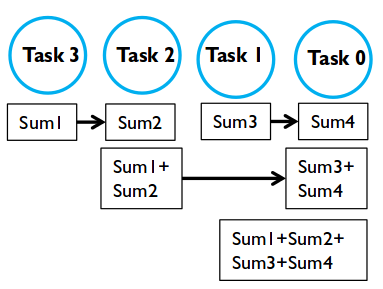
\includegraphics[scale=0.50]{reduce.png} 
\caption{Esquema de cómo \textsf{MPI\_REDUCE} funciona.} 
\label{fig:reduce}
\end{figure}
El escalado del tiempo de cómputo con el número de partículas ha sido diferente en función de la máquina. En mi caso he usado mi portáti \ref{fig:workerii_ana} y el clúster cerqt2 \ref{fig:cerqt2_ana}.

\begin{figure}[h!]
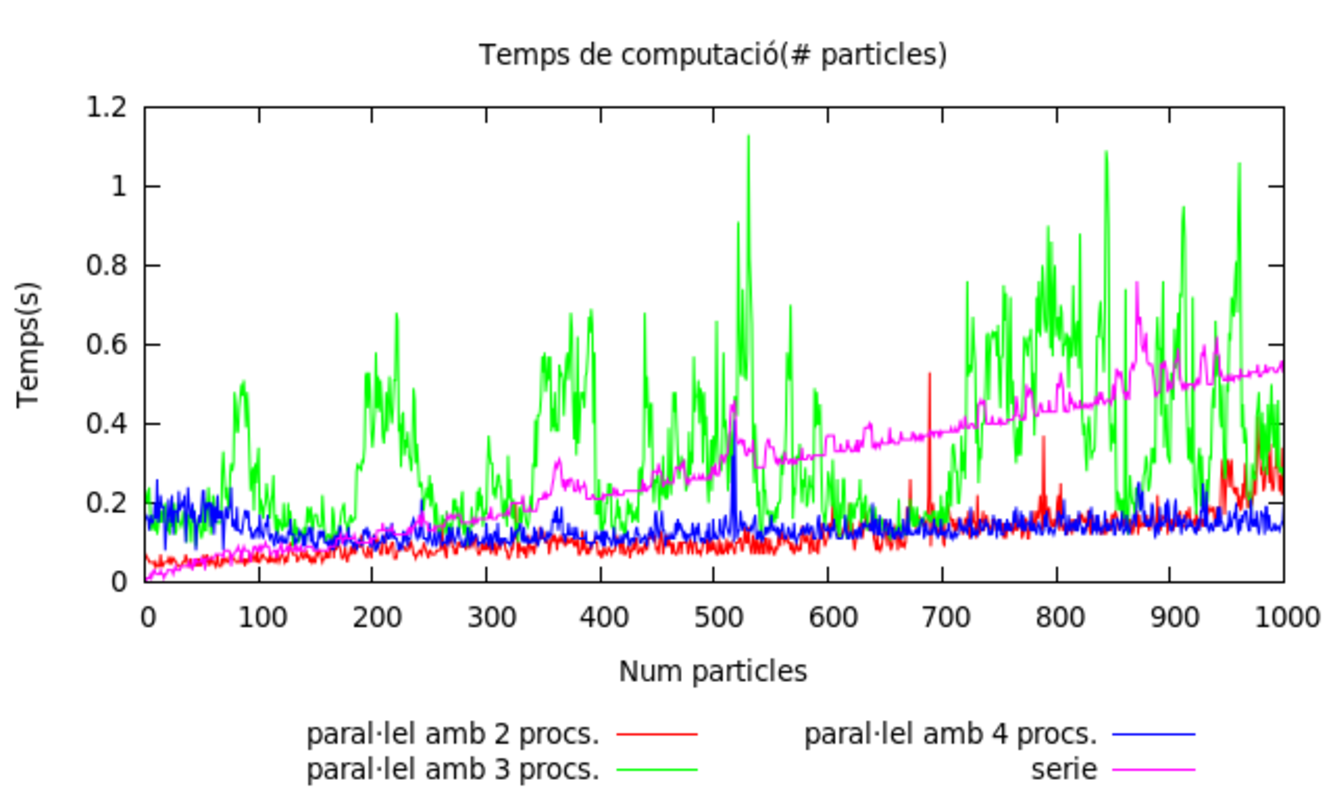
\includegraphics[scale=0.50]{bench_ana_workerII.pdf} 
\caption{Tiempo de cálculo (s) para diferente número de procesadores de los cálculos de presión y temperatura hechos en un portátil.} 
\label{fig:workerii_ana}
\end{figure}
\begin{figure}[h!]
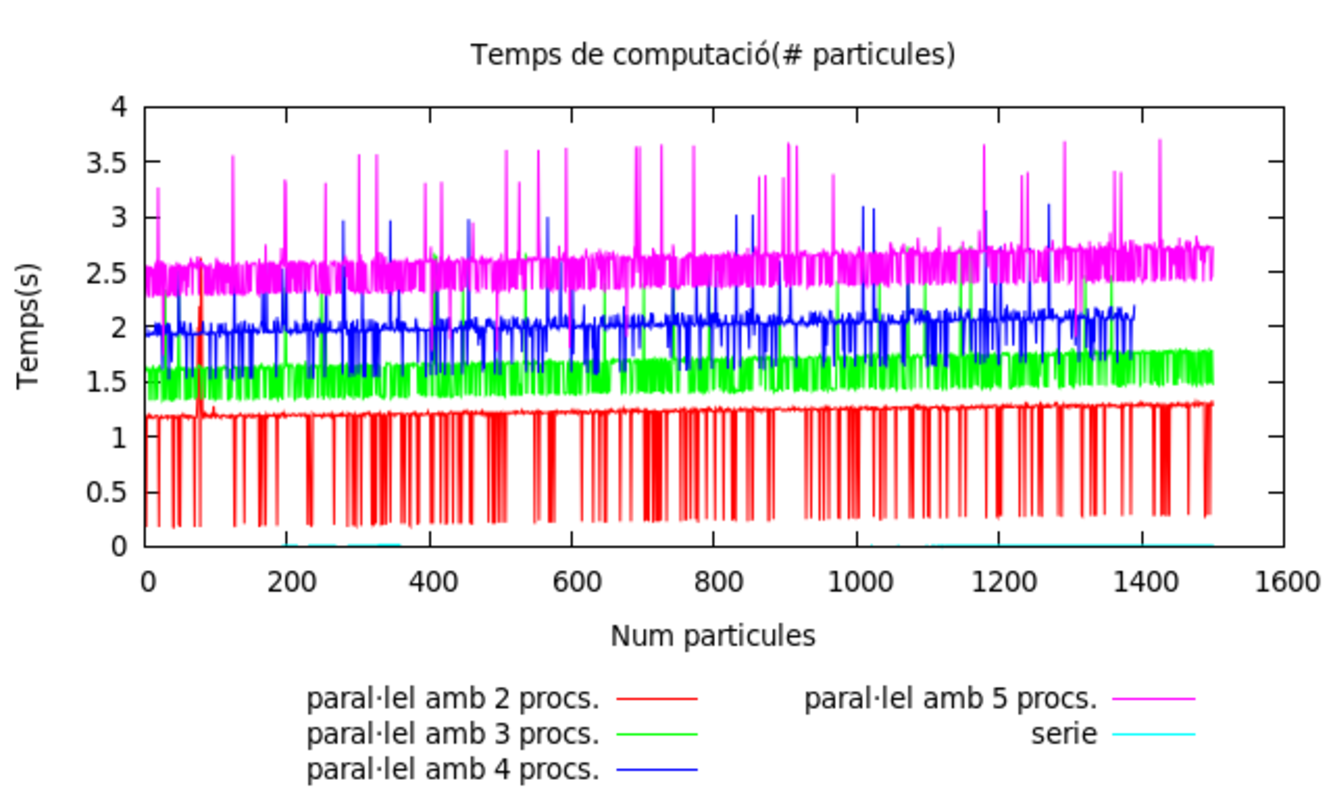
\includegraphics[scale=0.50]{bench_ana_cerqt2.pdf} 
\caption{Tiempo de cálculo (s) para diferente número de procesadores de los cálculos de presión y temperatura hechos en cerqt2.} 
\label{fig:cerqt2_ana}
\end{figure}
Lo curioso aquí, es que es mejor trabajar en un ordenador portátil con un número par de procesadores que en un clúster. Además, en el clúster oscila mucho el tiempo en función del número de partículas.

\subsection{Resultados}
Vemos en las figuras \ref{fig:tempe} y \ref{fig:presion}, que la temperatura y la presión llegan a un estado de equilibrio.
\begin{figure}[h!]
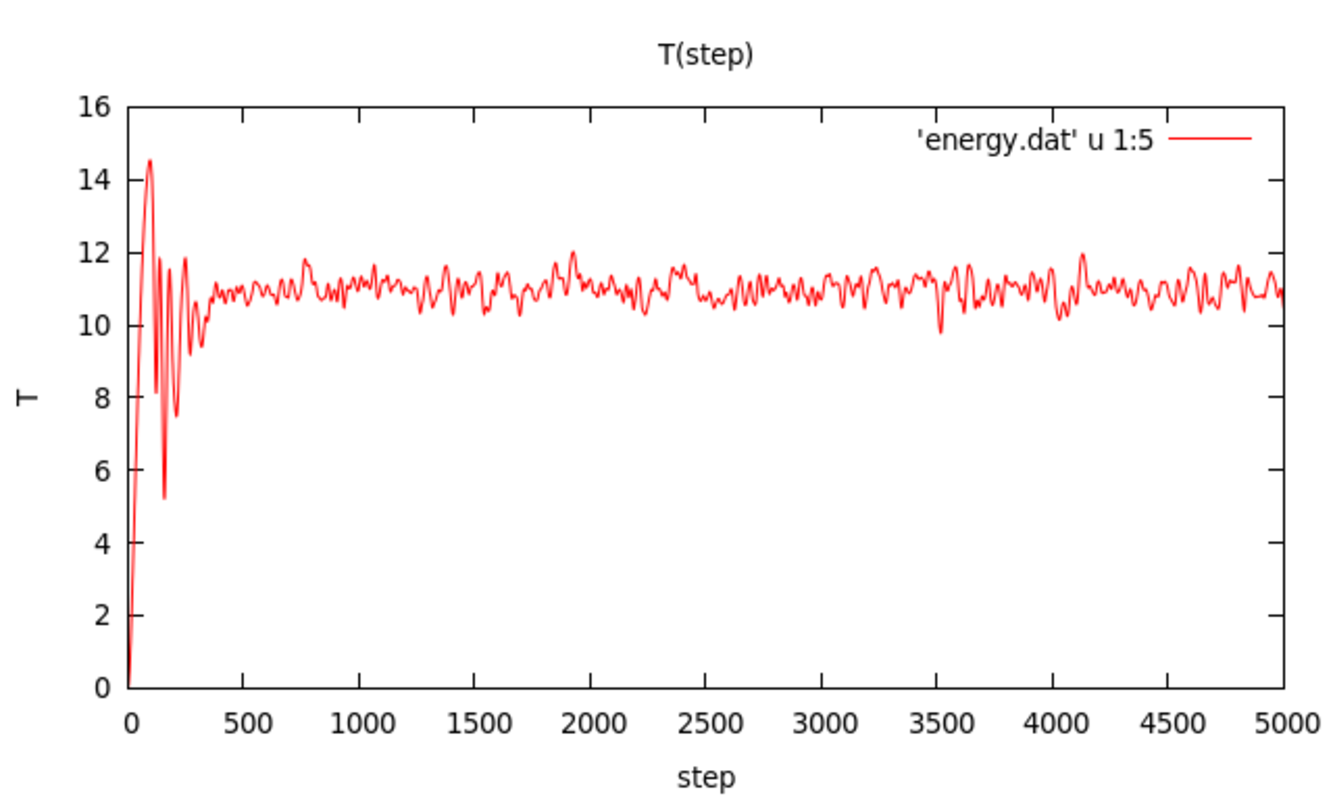
\includegraphics[scale=0.50]{temperatura.pdf} 
\caption{Temperatura en función del tiempo} 
\label{fig:tempe}
\end{figure}\begin{figure}[h!]
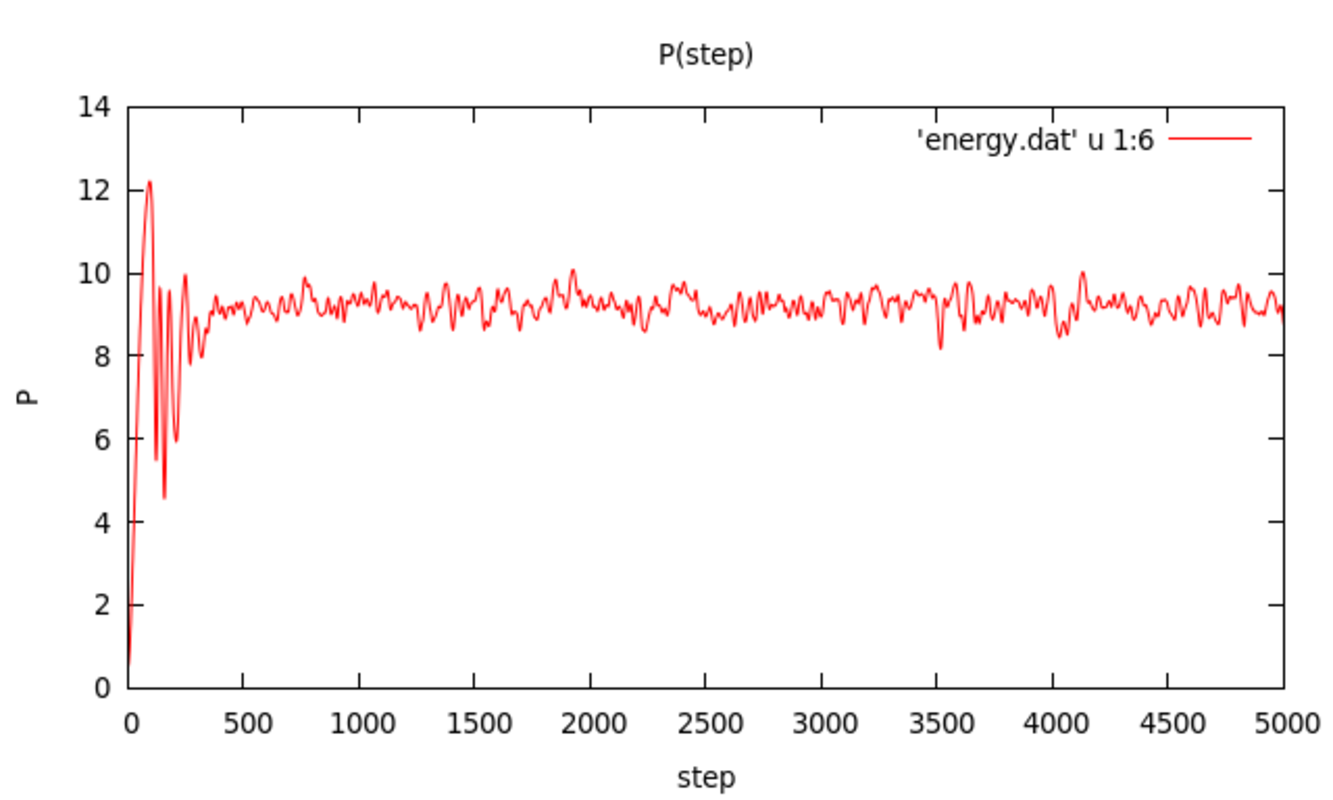
\includegraphics[scale=0.50]{presion.pdf} 
\caption{Presión en función del tiempo} 
\label{fig:presion}
\end{figure}


\subsection{Presión y temperatura:}
Para el cálculo de la presión hemos hecho uso del teorema del virial que nos relaciona el promedio del trabajo de todas las partículas (la energía potencial) con la energía cinética promedia.

\begin{equation}
\left\langle E_c \right\rangle= -\frac{1}{2} \left\langle \vec{F}^{\text{TOT}} \circ \vec{r} \right\rangle
\label{eq:virial}
\end{equation}

Descomponemos la fuerza total como la suma de la fuerza interna debido a la interacción entre partículas y la externa al sistema:

\begin{equation}
\vec{F}^{\text{TOT}} = \vec{F}^{\text{int}}+\vec{F}^{\text{ext}}
\end{equation}

Es promedio del trabajo de las fuerzas externas será debido a la presión que ejerce la caja. Descomponiendo por componentes, dicha fuerza externa obtenemos la relación del promedio del trabajo externo con la presión:
\begin{equation}
\left\langle W^{ext}	\right\rangle = L_x (-PL_yL_z)+L_y (-PL_xL_z)+L_z (-PL_xL_y)= -3PV
\end{equation}

Donde $L_x$ es el valor del lado $x$ de la caja (ídem para $L_y$ y $L_z$).

Utilizando el teorema de equipartición de la energía:
\begin{equation}
\left\langle E_c \right\rangle= \frac{3}{2} N k_B T
\label{eq:particion}
\end{equation}

en la ecuación \ref{eq:virial}, obtenemos que la presión vale:
\begin{equation}
P = \frac{Nk_BT}{V}+\frac{1}{3}\left\langle \vec{F}^{\text{int}} \circ \vec{r} \right\rangle
\label{eq:presion}
\end{equation}

Para la temperatura hemos usado el teorema de equipartición de la energía (eq. \ref{eq:particion}):
\begin{equation}
T = \frac{1}{3m} \left\langle \vec{v}^2 \right\rangle
\label{eq:temp}
\end{equation}

\subsection{Implementación:}
Viendo las expresiones \ref{eq:presion} y \ref{eq:temp}, podemos ver que por cada magnitud hay que hacer la suma de $N$ productos escalares y luego sumarles i/o multiplicar unas constantes. Así que la implementación del cálculo de ambas magnitudes son muy parecidas.

En términos de paralelización, lo que he hecho es hacer que cada procesador me coja el mismo número de partículas a excepción del último que me cogerá el resto que queden. Luego lo que hará cada procesador será la suma parcial de dichos productos escalares y luego con la subrutina \textsf{MPI\_REDUCE} las sumaré a un procesador común de manera jerárquica \ref{fig:reduce}.
\begin{figure}[H]
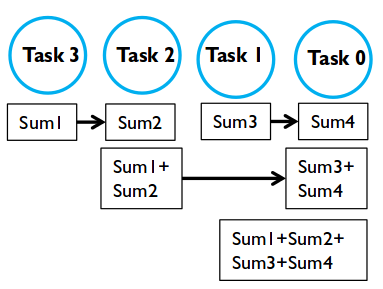
\includegraphics[scale=0.50]{reduce.png} 
\caption{Esquema de cómo \textsf{MPI\_REDUCE} funciona.} 
\label{fig:reduce}
\end{figure}
El escalado del tiempo de cómputo con el número de partículas ha sido diferente en función de la máquina. En mi caso he usado mi portáti \ref{fig:workerii_ana} y el clúster cerqt2 \ref{fig:cerqt2_ana}.

\begin{figure}[h!]
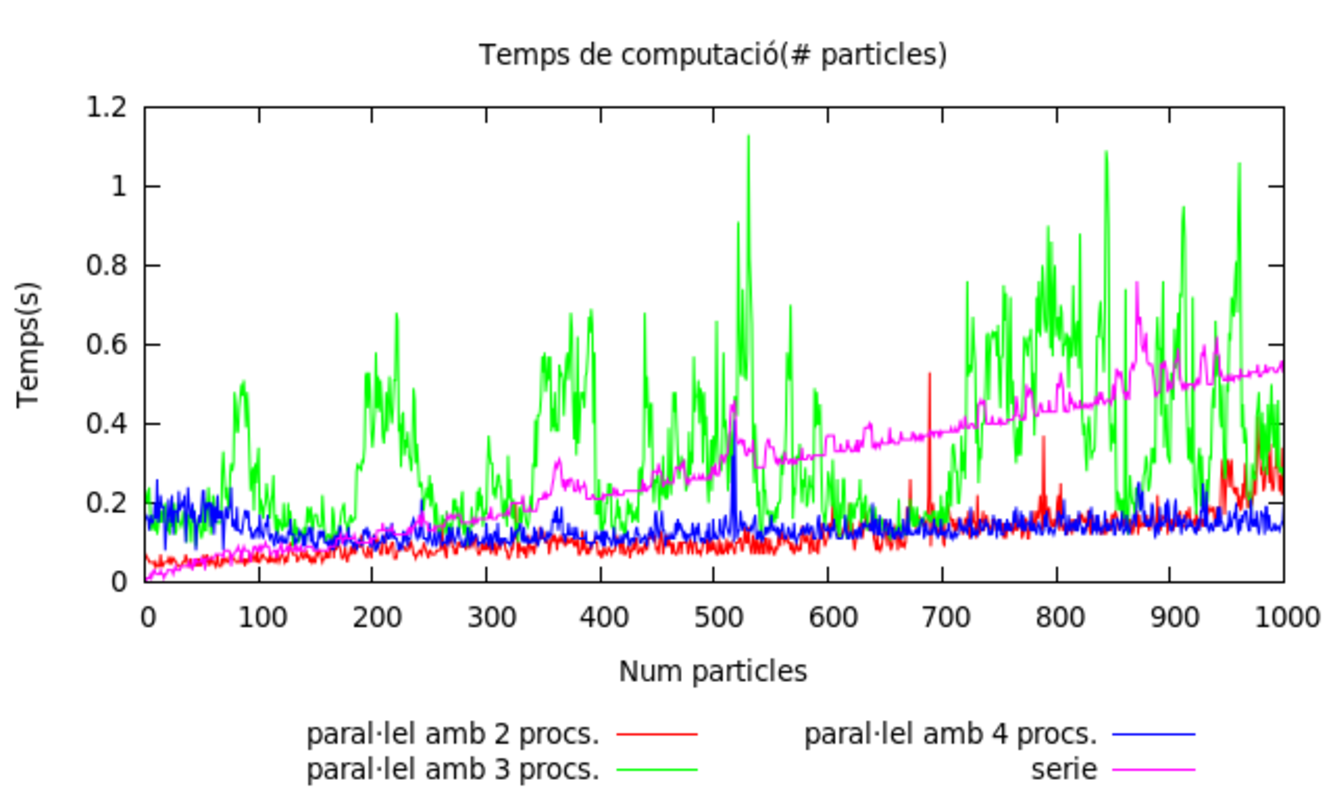
\includegraphics[scale=0.50]{bench_ana_workerII.pdf} 
\caption{Tiempo de cálculo (s) para diferente número de procesadores de los cálculos de presión y temperatura hechos en un portátil.} 
\label{fig:workerii_ana}
\end{figure}
\begin{figure}[h!]
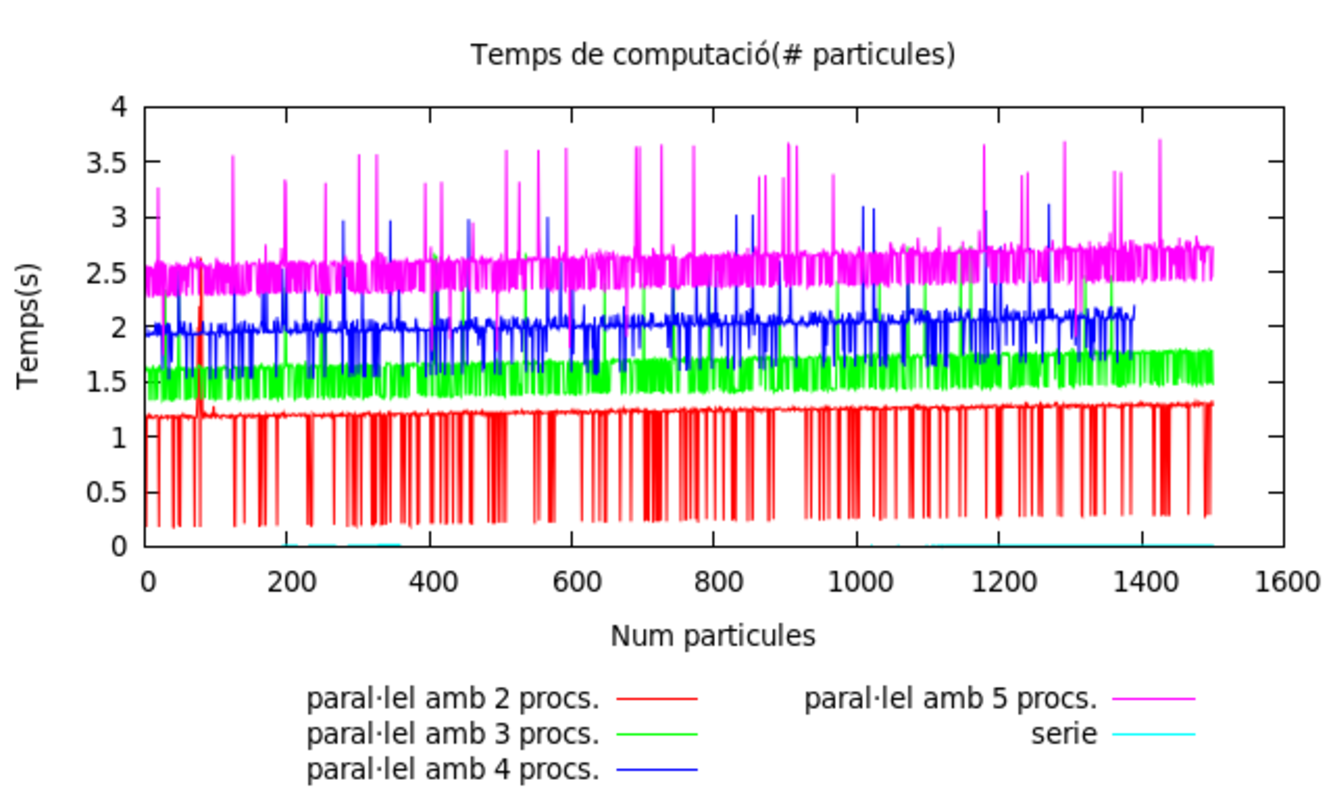
\includegraphics[scale=0.50]{bench_ana_cerqt2.pdf} 
\caption{Tiempo de cálculo (s) para diferente número de procesadores de los cálculos de presión y temperatura hechos en cerqt2.} 
\label{fig:cerqt2_ana}
\end{figure}
Lo curioso aquí, es que es mejor trabajar en un ordenador portátil con un número par de procesadores que en un clúster. Además, en el clúster oscila mucho el tiempo en función del número de partículas.

\subsection{Resultados}
Vemos en las figuras \ref{fig:tempe} y \ref{fig:presion}, que la temperatura y la presión llegan a un estado de equilibrio.
\begin{figure}[h!]
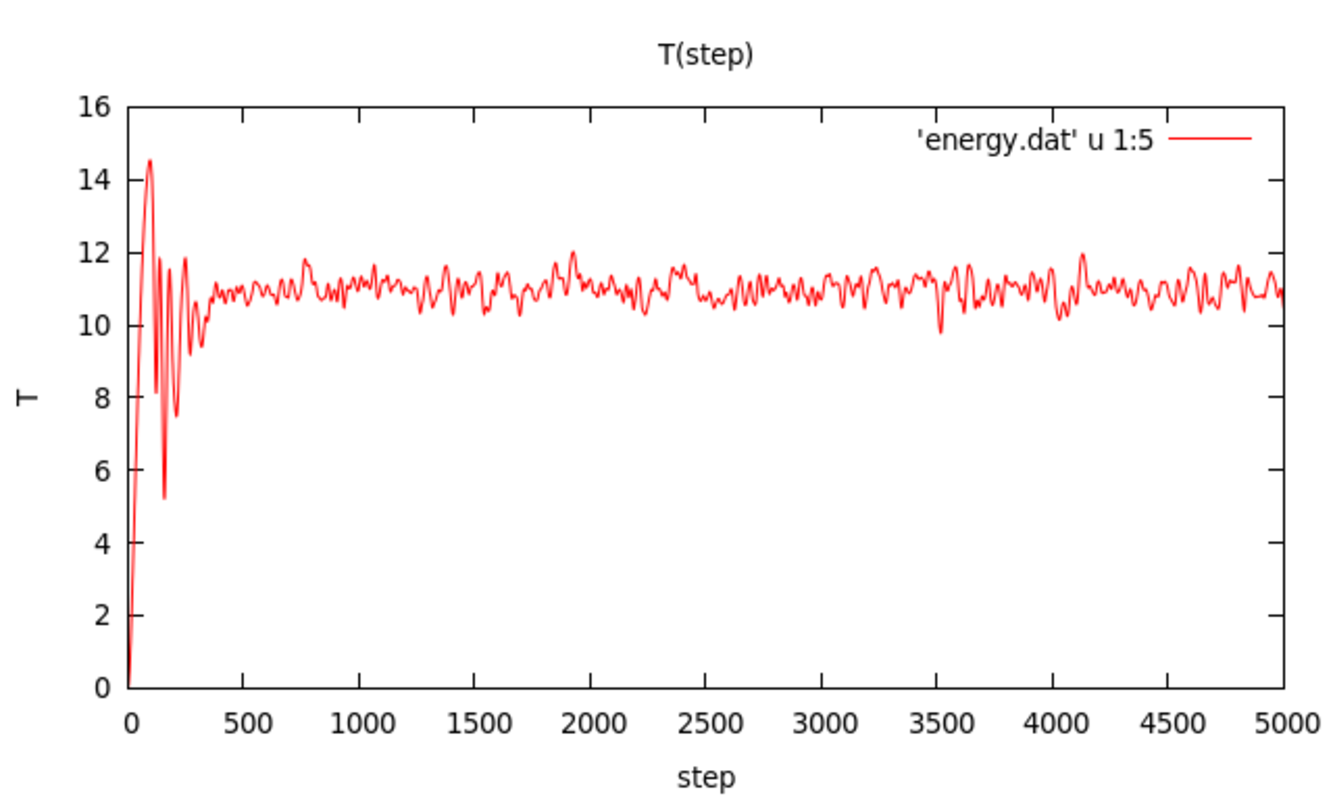
\includegraphics[scale=0.50]{temperatura.pdf} 
\caption{Temperatura en función del tiempo} 
\label{fig:tempe}
\end{figure}\begin{figure}[h!]
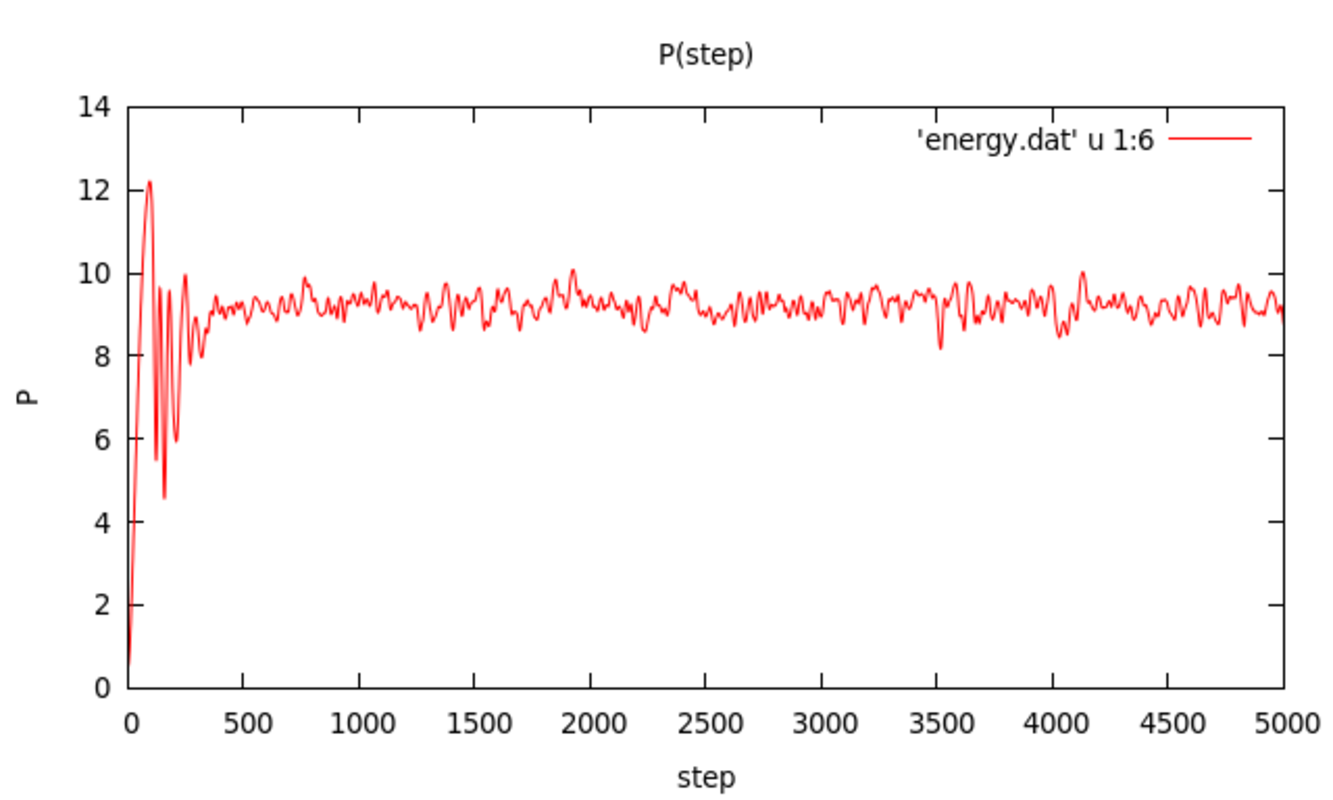
\includegraphics[scale=0.50]{presion.pdf} 
\caption{Presión en función del tiempo} 
\label{fig:presion}
\end{figure}


\subsection{Presión y temperatura:}
Para el cálculo de la presión hemos hecho uso del teorema del virial que nos relaciona el promedio del trabajo de todas las partículas (la energía potencial) con la energía cinética promedia.

\begin{equation}
\left\langle E_c \right\rangle= -\frac{1}{2} \left\langle \vec{F}^{\text{TOT}} \circ \vec{r} \right\rangle
\label{eq:virial}
\end{equation}

Descomponemos la fuerza total como la suma de la fuerza interna debido a la interacción entre partículas y la externa al sistema:

\begin{equation}
\vec{F}^{\text{TOT}} = \vec{F}^{\text{int}}+\vec{F}^{\text{ext}}
\end{equation}

Es promedio del trabajo de las fuerzas externas será debido a la presión que ejerce la caja. Descomponiendo por componentes, dicha fuerza externa obtenemos la relación del promedio del trabajo externo con la presión:
\begin{equation}
\left\langle W^{ext}	\right\rangle = L_x (-PL_yL_z)+L_y (-PL_xL_z)+L_z (-PL_xL_y)= -3PV
\end{equation}

Donde $L_x$ es el valor del lado $x$ de la caja (ídem para $L_y$ y $L_z$).

Utilizando el teorema de equipartición de la energía:
\begin{equation}
\left\langle E_c \right\rangle= \frac{3}{2} N k_B T
\label{eq:particion}
\end{equation}

en la ecuación \ref{eq:virial}, obtenemos que la presión vale:
\begin{equation}
P = \frac{Nk_BT}{V}+\frac{1}{3}\left\langle \vec{F}^{\text{int}} \circ \vec{r} \right\rangle
\label{eq:presion}
\end{equation}

Para la temperatura hemos usado el teorema de equipartición de la energía (eq. \ref{eq:particion}):
\begin{equation}
T = \frac{1}{3m} \left\langle \vec{v}^2 \right\rangle
\label{eq:temp}
\end{equation}

\subsection{Implementación:}
Viendo las expresiones \ref{eq:presion} y \ref{eq:temp}, podemos ver que por cada magnitud hay que hacer la suma de $N$ productos escalares y luego sumarles i/o multiplicar unas constantes. Así que la implementación del cálculo de ambas magnitudes son muy parecidas.

En términos de paralelización, lo que he hecho es hacer que cada procesador me coja el mismo número de partículas a excepción del último que me cogerá el resto que queden. Luego lo que hará cada procesador será la suma parcial de dichos productos escalares y luego con la subrutina \textsf{MPI\_REDUCE} las sumaré a un procesador común de manera jerárquica \ref{fig:reduce}.
\begin{figure}[H]
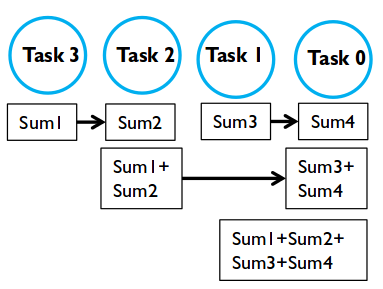
\includegraphics[scale=0.50]{reduce.png} 
\caption{Esquema de cómo \textsf{MPI\_REDUCE} funciona.} 
\label{fig:reduce}
\end{figure}
El escalado del tiempo de cómputo con el número de partículas ha sido diferente en función de la máquina. En mi caso he usado mi portáti \ref{fig:workerii_ana} y el clúster cerqt2 \ref{fig:cerqt2_ana}.

\begin{figure}[h!]
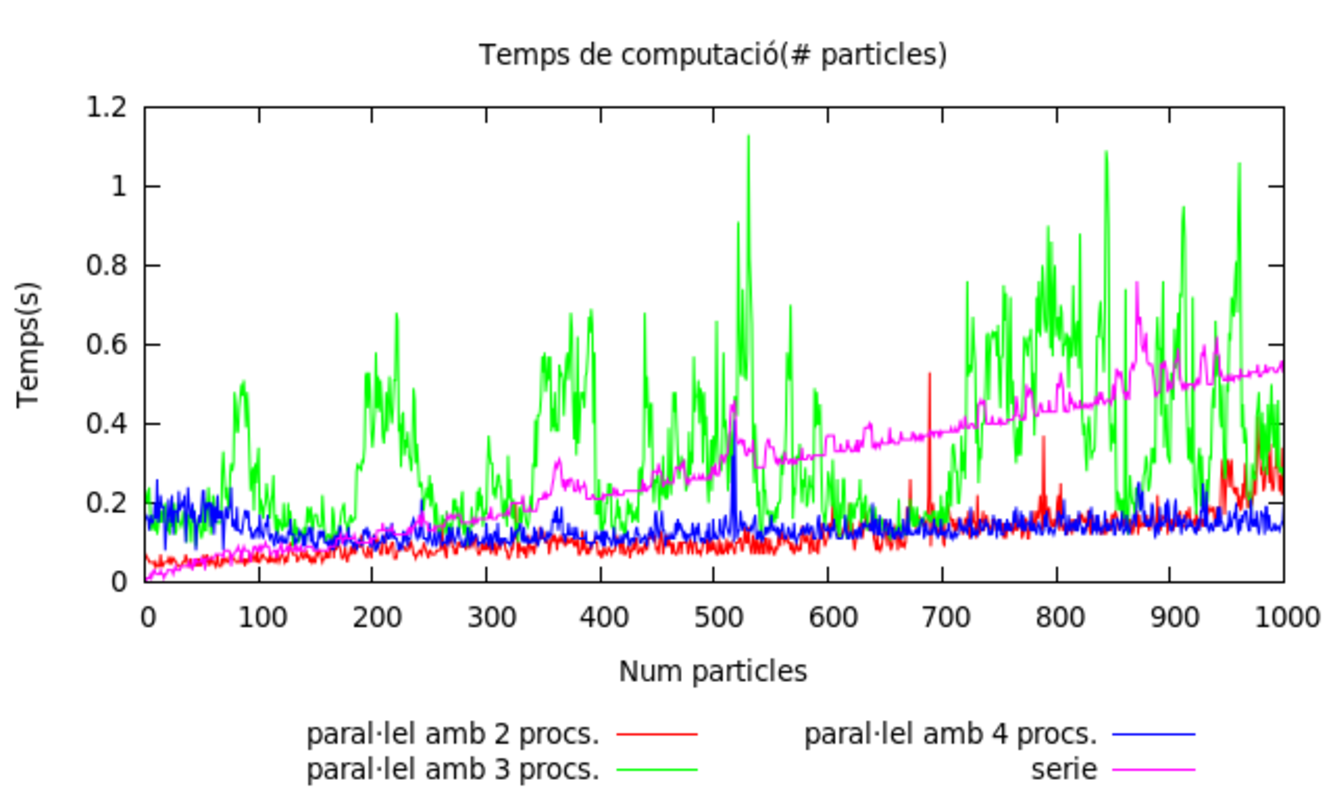
\includegraphics[scale=0.50]{bench_ana_workerII.pdf} 
\caption{Tiempo de cálculo (s) para diferente número de procesadores de los cálculos de presión y temperatura hechos en un portátil.} 
\label{fig:workerii_ana}
\end{figure}
\begin{figure}[h!]
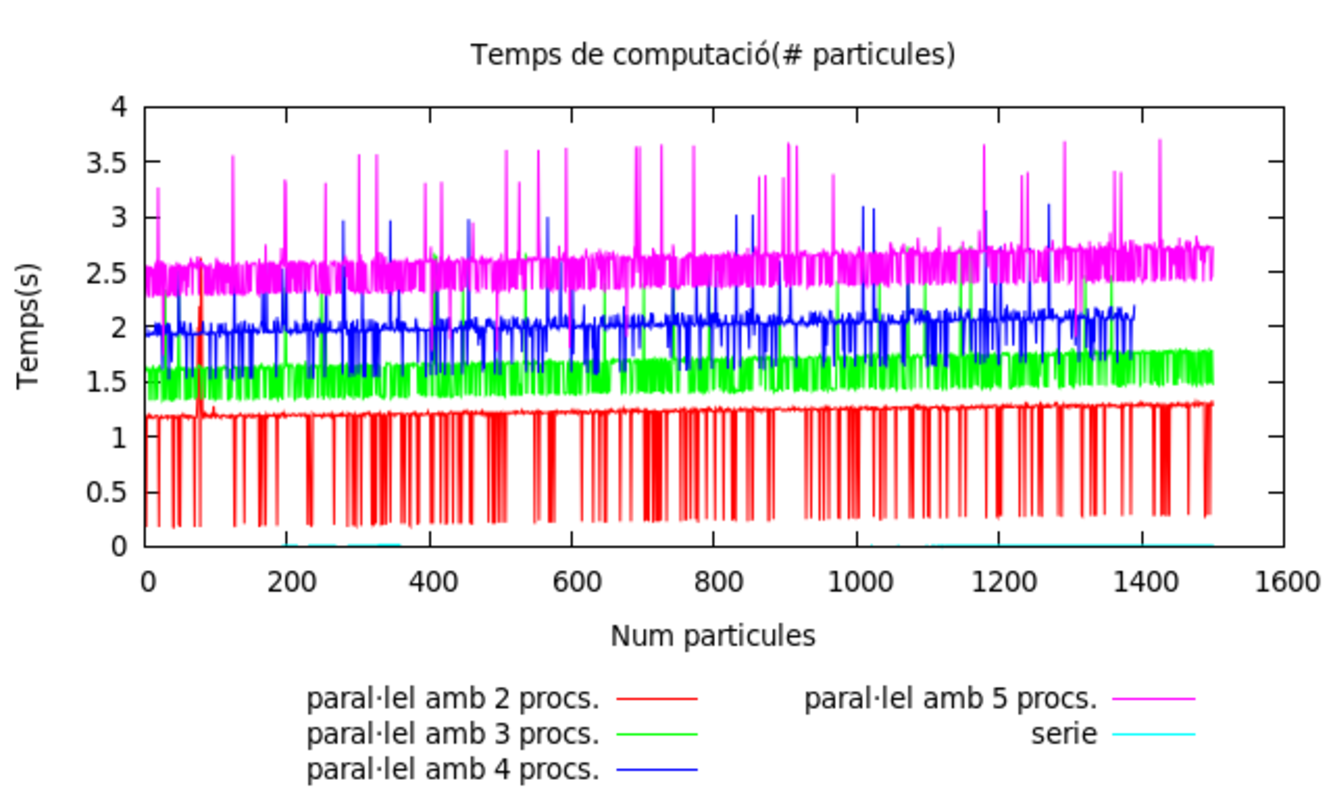
\includegraphics[scale=0.50]{bench_ana_cerqt2.pdf} 
\caption{Tiempo de cálculo (s) para diferente número de procesadores de los cálculos de presión y temperatura hechos en cerqt2.} 
\label{fig:cerqt2_ana}
\end{figure}
Lo curioso aquí, es que es mejor trabajar en un ordenador portátil con un número par de procesadores que en un clúster. Además, en el clúster oscila mucho el tiempo en función del número de partículas.

\subsection{Resultados}
Vemos en las figuras \ref{fig:tempe} y \ref{fig:presion}, que la temperatura y la presión llegan a un estado de equilibrio.
\begin{figure}[h!]
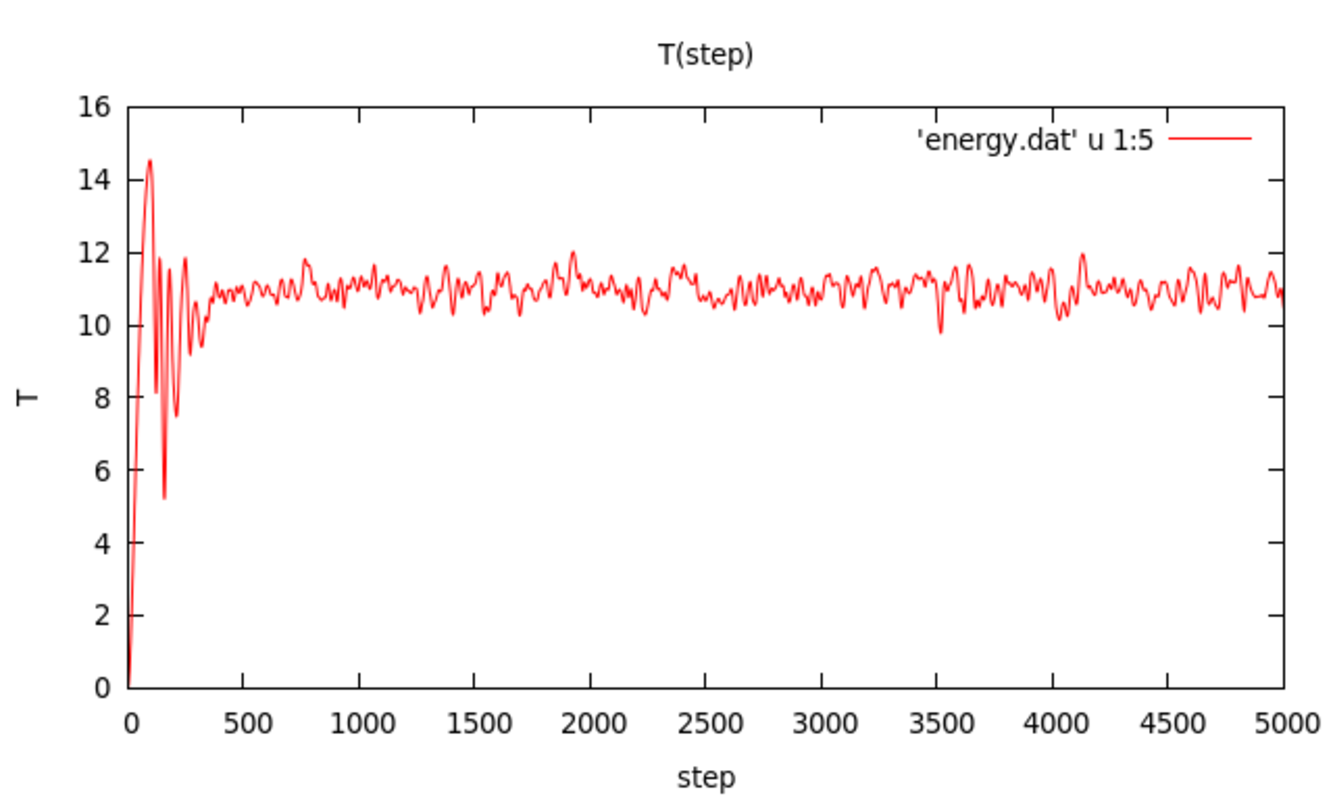
\includegraphics[scale=0.50]{temperatura.pdf} 
\caption{Temperatura en función del tiempo} 
\label{fig:tempe}
\end{figure}\begin{figure}[h!]
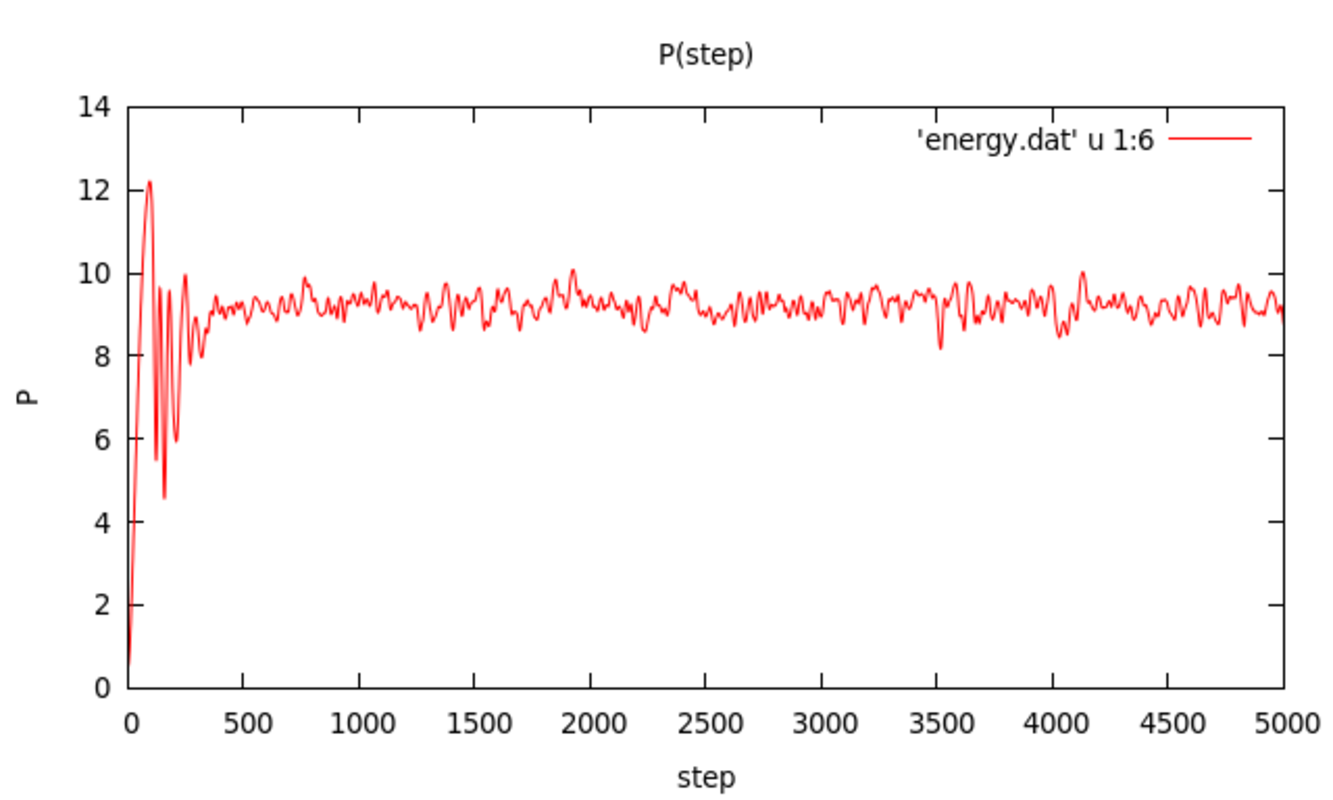
\includegraphics[scale=0.50]{presion.pdf} 
\caption{Presión en función del tiempo} 
\label{fig:presion}
\end{figure}


\subsection{Presión y temperatura:}
Para el cálculo de la presión hemos hecho uso del teorema del virial que nos relaciona el promedio del trabajo de todas las partículas (la energía potencial) con la energía cinética promedia.

\begin{equation}
\left\langle E_c \right\rangle= -\frac{1}{2} \left\langle \vec{F}^{\text{TOT}} \circ \vec{r} \right\rangle
\label{eq:virial}
\end{equation}

Descomponemos la fuerza total como la suma de la fuerza interna debido a la interacción entre partículas y la externa al sistema:

\begin{equation}
\vec{F}^{\text{TOT}} = \vec{F}^{\text{int}}+\vec{F}^{\text{ext}}
\end{equation}

Es promedio del trabajo de las fuerzas externas será debido a la presión que ejerce la caja. Descomponiendo por componentes, dicha fuerza externa obtenemos la relación del promedio del trabajo externo con la presión:
\begin{equation}
\left\langle W^{ext}	\right\rangle = L_x (-PL_yL_z)+L_y (-PL_xL_z)+L_z (-PL_xL_y)= -3PV
\end{equation}

Donde $L_x$ es el valor del lado $x$ de la caja (ídem para $L_y$ y $L_z$).

Utilizando el teorema de equipartición de la energía:
\begin{equation}
\left\langle E_c \right\rangle= \frac{3}{2} N k_B T
\label{eq:particion}
\end{equation}

en la ecuación \ref{eq:virial}, obtenemos que la presión vale:
\begin{equation}
P = \frac{Nk_BT}{V}+\frac{1}{3}\left\langle \vec{F}^{\text{int}} \circ \vec{r} \right\rangle
\label{eq:presion}
\end{equation}

Para la temperatura hemos usado el teorema de equipartición de la energía (eq. \ref{eq:particion}):
\begin{equation}
T = \frac{1}{3m} \left\langle \vec{v}^2 \right\rangle
\label{eq:temp}
\end{equation}

\subsection{Implementación:}
Viendo las expresiones \ref{eq:presion} y \ref{eq:temp}, podemos ver que por cada magnitud hay que hacer la suma de $N$ productos escalares y luego sumarles i/o multiplicar unas constantes. Así que la implementación del cálculo de ambas magnitudes son muy parecidas.

En términos de paralelización, lo que he hecho es hacer que cada procesador me coja el mismo número de partículas a excepción del último que me cogerá el resto que queden. Luego lo que hará cada procesador será la suma parcial de dichos productos escalares y luego con la subrutina \textsf{MPI\_REDUCE}.
\begin{figure}[H]
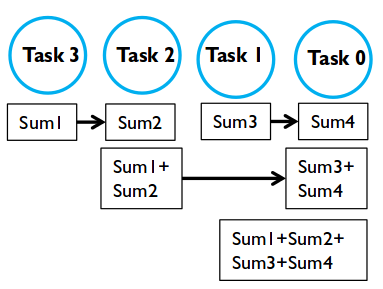
\includegraphics[scale=0.50]{reduce.png} 
\caption{Esquema de cómo \textsf{MPI\_REDUCE} funciona.} 
\label{fig:cerqt2_ana}
\end{figure}
El escalado del tiempo de cómputo con el número de partículas ha sido diferente en función de la máquina. En mi caso he usado mi portáti \ref{fig:workerii_ana} y el clúster cerqt2 \ref{fig:cerqt2_ana}.

\begin{figure}[h!]
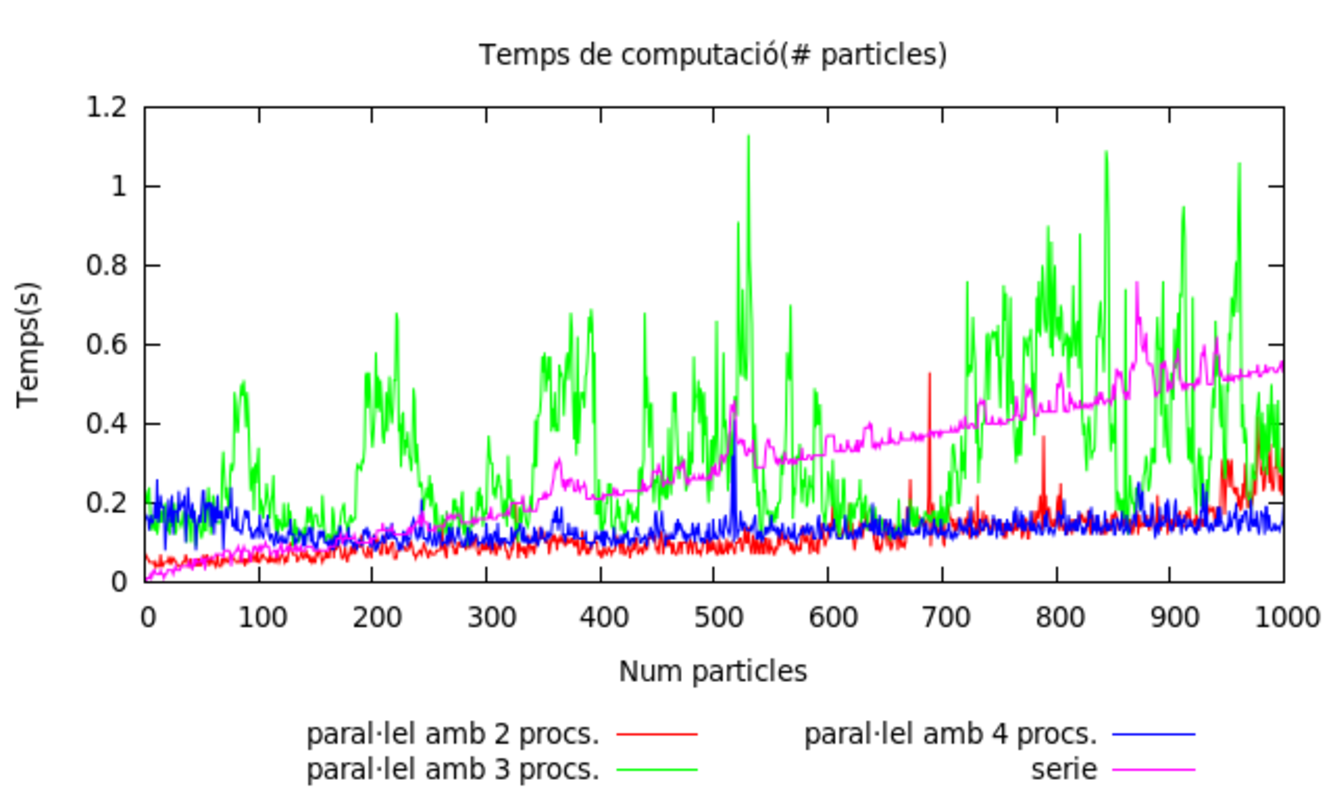
\includegraphics[scale=0.50]{bench_ana_workerII.pdf} 
\caption{Tiempo de cálculo (s) para diferente número de procesadores de los cálculos de presión y temperatura hechos en un portátil.} 
\label{fig:workerii_ana}
\end{figure}
\begin{figure}[h!]
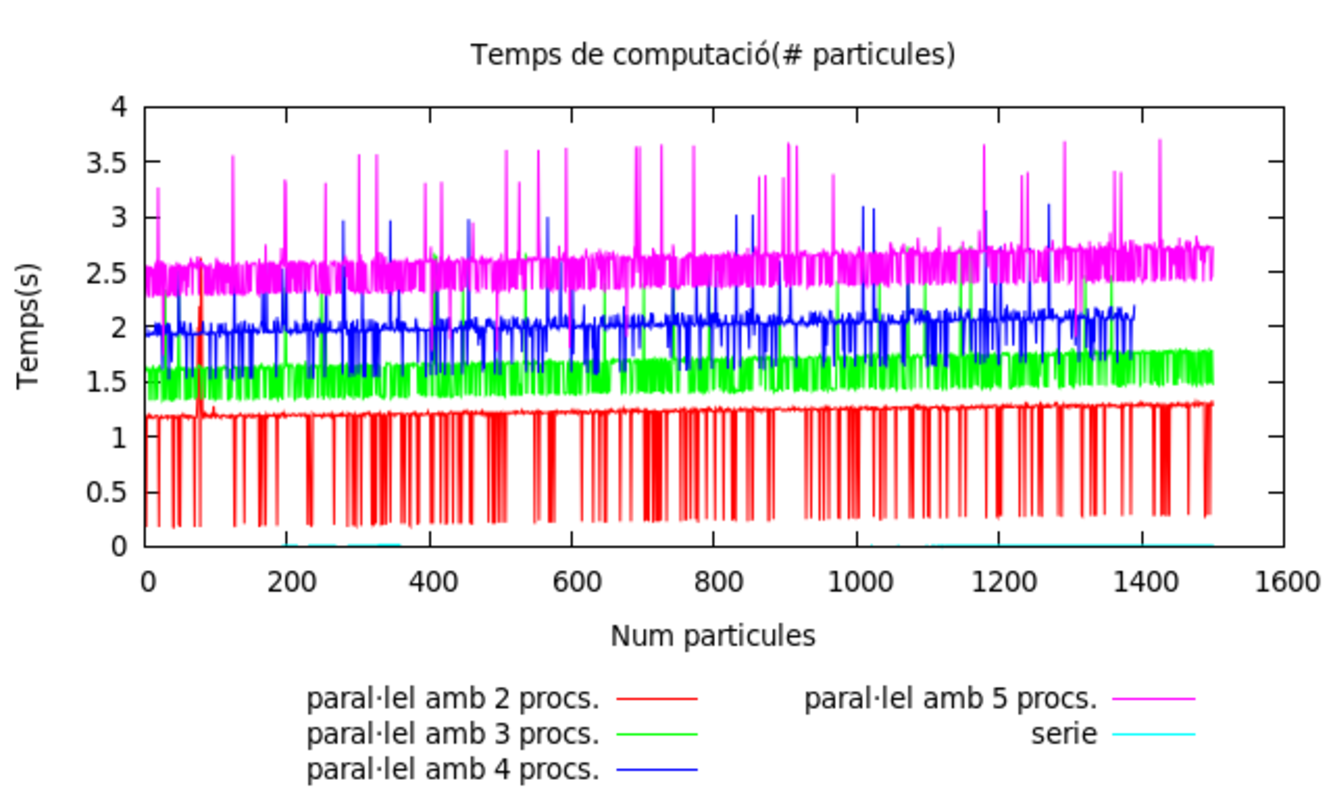
\includegraphics[scale=0.50]{bench_ana_cerqt2.pdf} 
\caption{Tiempo de cálculo (s) para diferente número de procesadores de los cálculos de presión y temperatura hechos en cerqt2.} 
\label{fig:cerqt2_ana}
\end{figure}
Lo curioso aquí, es que es mejor trabajar en un ordenador portátil con un número par de procesadores que en un clúster. Además, en el clúster oscila mucho el tiempo en función del número de partículas.

\subsection{Resultados}
Vemos en las figuras \ref{fig:tempe} y \ref{fig:presion}, que la temperatura y la presión llegan a un estado de equilibrio.
\begin{figure}[h!]
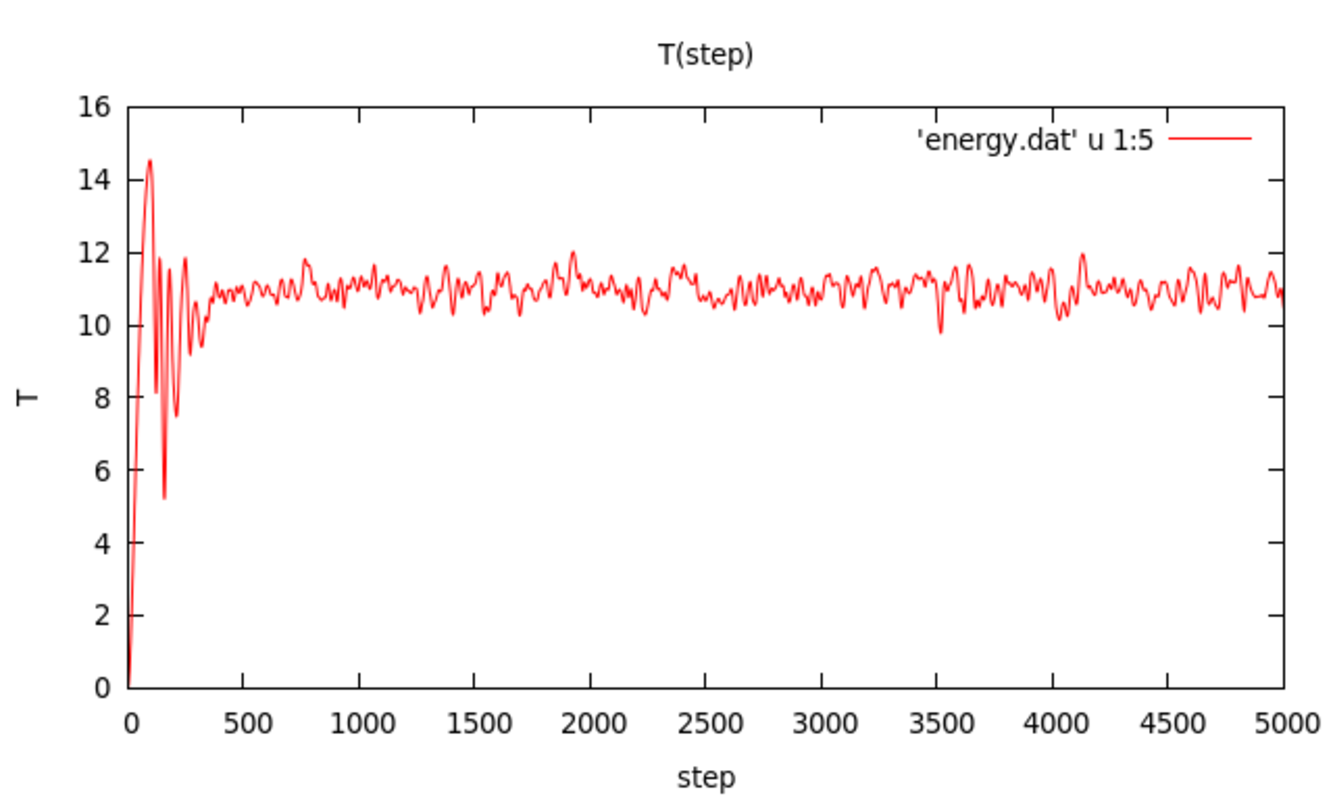
\includegraphics[scale=0.50]{temperatura.pdf} 
\caption{Temperatura en función del tiempo} 
\label{fig:tempe}
\end{figure}\begin{figure}[h!]
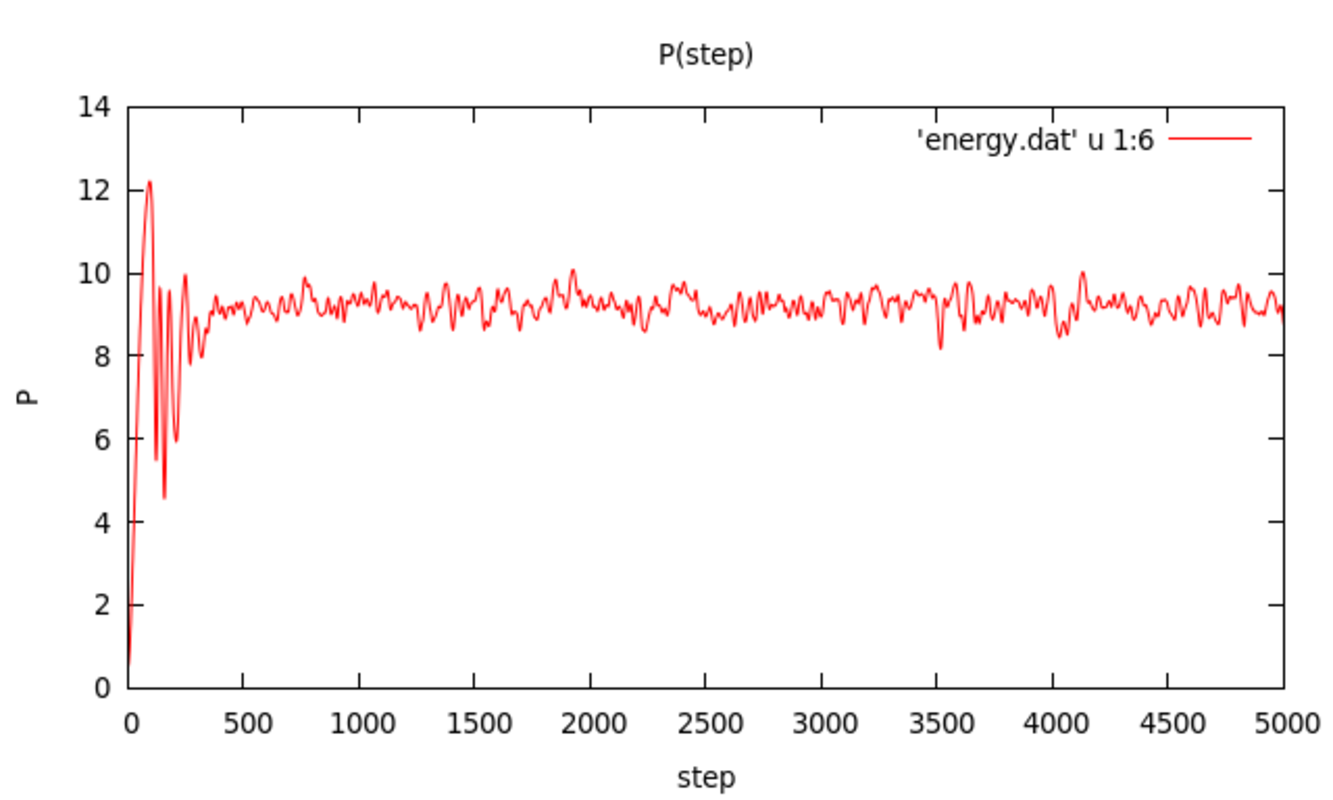
\includegraphics[scale=0.50]{presion.pdf} 
\caption{Presión en función del tiempo} 
\label{fig:presion}
\end{figure}